\documentclass[9pt]{beamer}
\usetheme{default}
\usecolortheme{default}

% Reduce margins
\setbeamersize{text margin left=0.6cm, text margin right=0.6cm}

% Packages
\usepackage{amsmath, amssymb, bm}
\usepackage{graphicx}
\usepackage{tikz}
\usetikzlibrary{arrows.meta, positioning}

% Colors
\definecolor{slideblue}{RGB}{0, 102, 153}
\setbeamercolor{frametitle}{fg=slideblue}
\setbeamercolor{title}{fg=slideblue}
\setbeamercolor{structure}{fg=slideblue}
\setbeamercolor{alerted text}{fg=red}

% Tighter itemize spacing
\setlength{\leftmargini}{1em}
\setlength{\leftmarginii}{1em}

% Footer
\setbeamertemplate{footline}{%
  \leavevmode%
  \hbox{%
    \begin{beamercolorbox}[wd=.33\paperwidth,ht=2.25ex,dp=1ex,left]{author in head/foot}%
      \usebeamerfont{author in head/foot}\hspace{1em}ECON712
    \end{beamercolorbox}%
    \begin{beamercolorbox}[wd=.34\paperwidth,ht=2.25ex,dp=1ex,center]{title in head/foot}%
      \usebeamerfont{title in head/foot}Winter 2026
    \end{beamercolorbox}%
    \begin{beamercolorbox}[wd=.33\paperwidth,ht=2.25ex,dp=1ex,right]{date in head/foot}%
      \usebeamerfont{date in head/foot}Lectures 14\hspace{1em}
      \insertframenumber{} / \inserttotalframenumber\hspace{1em}
    \end{beamercolorbox}}%
  \vskip0pt%
}
\setbeamertemplate{navigation symbols}{}

\title{ECON 712: Applied Econometrics\\[0.3em]
       Lecture 14: Introduction to Instrumental Variables}
\date{ECON712 Winter 2026}

\begin{document}

% ------------------------------------------------------------------
\begin{frame}
  \titlepage
\end{frame}

% ------------------------------------------------------------------
\begin{frame}{Instrumental Variables}
  \begin{itemize}
    \item There are instances where we cannot solve endogeneity by adding controls, e.g.
    \begin{itemize}
      \item[$\blacktriangleright$] Omitted variable bias: the omitted variable is not observed
      \item[$\blacktriangleright$] Treatment Effects: treatment assignment does not satisfy the CIA assumption for any set of observable covariates
    \end{itemize}
    \medskip
    \item We can solve this by finding an instrument $Z$ that allows us to identify the causal effect of an endogenous variable $X$
    \begin{itemize}
      \item[$\blacktriangleright$] An instrument only affects the outcome variable through $X$ and does not correlate with unobserved variables affecting the outcome
    \end{itemize}
  \end{itemize}
\end{frame}

% ------------------------------------------------------------------
\begin{frame}{E.g.\ Omitted Variable Bias}
  \begin{itemize}
    \item Suppose the true causal model is:
  \end{itemize}
  \begin{center}
  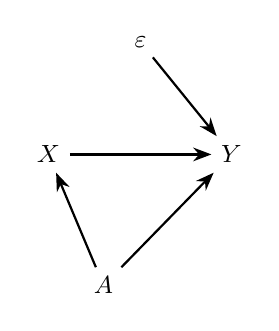
\begin{tikzpicture}[node distance=1.5cm, every node/.style={font=\small},
                      arr/.style={-{Stealth}, thick}]
    \node (eps) {$\varepsilon$};
    \node (X) [below left=1.0cm and 0.7cm of eps] {$X$};
    \node (Y) [below right=1.0cm and 0.7cm of eps] {$Y$};
    \node (A) [below=1.2cm of X, xshift=0.7cm] {$A$};
    \draw[arr] (eps)--(Y); \draw[arr] (X)--(Y);
    \draw[arr] (A)--(X);   \draw[arr] (A)--(Y);
  \end{tikzpicture}
  \end{center}
  \begin{itemize}
    \item[$\blacktriangleright$] This gives: $y = \beta_0 + \beta_1 x + \beta_2 A + \epsilon$
  \end{itemize}
  \medskip
  \begin{itemize}
    \item An instrument $z$ satisfies:
  \end{itemize}
  \begin{center}
  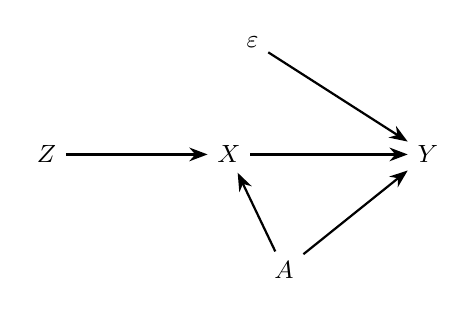
\begin{tikzpicture}[node distance=1.5cm, every node/.style={font=\small},
                      arr/.style={-{Stealth}, thick}]
    \node (eps) {$\varepsilon$};
    \node (X) [below=1.0cm of eps, xshift=-0.3cm] {$X$};
    \node (Y) [right=2.0cm of X] {$Y$};
    \node (Z) [left=1.8cm of X] {$Z$};
    \node (A) [below=1.0cm of X, xshift=0.7cm] {$A$};
    \draw[arr] (eps)--(Y); \draw[arr] (Z)--(X);
    \draw[arr] (X)--(Y);   \draw[arr] (A)--(X); \draw[arr] (A)--(Y);
  \end{tikzpicture}
  \end{center}
\end{frame}

% ------------------------------------------------------------------
\begin{frame}{E.g.\ Omitted Variable Bias}
  \begin{itemize}
    \item OLS on $y = \beta_0 + \beta_1 x + \eta$ (where $\eta = \beta_2 A + \epsilon$) gives a \textbf{biased and inconsistent} estimator.
    \medskip
    \item However: (i) $\mathrm{Cov}(z,x)\neq 0$, \;(ii) $\mathrm{Cov}(z,\eta)=0$ (\textcolor{slideblue}{exclusion restriction}), \;(iii) $z$ only affects $y$ through $x$
    \begin{itemize}
      \item[$\blacktriangleright$] \textbf{Q:} If we observe $z$, can we estimate $\beta_1$? \;\textcolor{slideblue}{\textbf{YES}}
    \end{itemize}
    \medskip
    \item Using the reduced-form and first-stage:
    \[
      \beta_1 = \frac{\mathrm{Cov}(y,z)}{\mathrm{Cov}(x,z)} = \frac{\gamma_1}{\alpha_1}
    \]
    \begin{align*}
      y &= \gamma_0 + \gamma_1 z + u, \quad E[u|z]=0 \quad \text{(Reduced-Form)}\\
      x &= \alpha_0 + \alpha_1 z + \nu, \quad E[\nu|z]=0 \quad \text{(First-Stage)}
    \end{align*}
  \end{itemize}
\end{frame}

% ------------------------------------------------------------------
\begin{frame}{IV Estimate}
  \begin{itemize}
    \item Sample analogue:
    \[
      \hat{\beta}_1^{IV} = \frac{\hat{\gamma}_1}{\hat{\alpha}_1}, \quad
      \hat{\gamma}_1 = \frac{\sum_{i}(y_i-\bar{y})(z_i-\bar{z})}{\sum_{i}(z_i-\bar{z})^2}, \quad
      \hat{\alpha}_1 = \frac{\sum_{i}(x_i-\bar{x})(z_i-\bar{z})}{\sum_{i}(z_i-\bar{z})^2}
    \]
    \medskip
    \item We \textbf{cannot} show unbiasedness in finite samples, but we can show consistency:
    \[
      \mathrm{plim}\!\left(\hat{\beta}_1^{IV} - \beta_1\right)
      = \frac{\mathrm{plim}\,\frac{1}{n}\sum_{i}(z_i-\bar{z})\,\eta_i}
             {\mathrm{plim}\,\frac{1}{n}\sum_{i}(x_i-\bar{x})(z_i-\bar{z})}
      = \frac{\mathrm{Corr}(z,\eta)\,\sigma_\eta}{\mathrm{Corr}(x,z)\,\sigma_x} = 0
    \]
  \end{itemize}
\end{frame}

% ------------------------------------------------------------------
% Slide 6a: 2SLS — General form
% ------------------------------------------------------------------
\begin{frame}{2SLS: General Vector Form}

  \textbf{Setup.} Partition regressors into exogenous controls $\mathbf{S}$ ($n\times k$) and one endogenous variable $\mathbf{x}$ ($n\times 1$):
  \[
    \mathbf{y} = \mathbf{S}\bm{\delta} + \mathbf{x}\beta_1 + \bm{\eta}
    \;\equiv\; \mathbf{X}\bm{\beta} + \bm{\eta},
    \qquad \mathbf{X} = [\,\mathbf{S}\;\;\mathbf{x}\,] \in \mathbb{R}^{n\times(k+1)}
  \]
  Stack exogenous controls and $j$ excluded instruments into the instrument matrix:
  \[
    \mathbf{Z} = [\,\mathbf{S}\;\;\mathbf{Z}_{\!2}\,] \in \mathbb{R}^{n\times(k+j)}
  \]

  \medskip
  \textbf{Order condition (necessary for identification):}
  \[
    j \geq 1
    \;\Longleftrightarrow\;
    \underbrace{k+j}_{\text{\# instruments}} \;\geq\; \underbrace{k+1}_{\text{\# regressors}}
  \]
  \begin{itemize}
    \item $j=1$: \textcolor{slideblue}{just-identified} \quad $j>1$: overidentified \quad \alert{$j<1$: underidentified --- \textbf{cannot estimate} $\beta_1$}
  \end{itemize}

  \medskip
  \textbf{2SLS estimator.} Let $\mathbf{P}_Z = \mathbf{Z}(\mathbf{Z}^\top\mathbf{Z})^{-1}\mathbf{Z}^\top$:
  \[
    \boxed{
      \hat{\bm{\beta}}^{2SLS}
      = \bigl(\mathbf{X}^\top \mathbf{P}_Z \mathbf{X}\bigr)^{-1}
        \mathbf{X}^\top \mathbf{P}_Z \mathbf{y}
    }
  \]
  Intuitively, $\mathbf{P}_Z\mathbf{X}$ purges $\mathbf{x}$ of its endogenous component, keeping only the variation attributable to $\mathbf{Z}$.

\end{frame}

% ------------------------------------------------------------------
% Slide 6b: Just-identified + FWL
% ------------------------------------------------------------------
\begin{frame}{2SLS: Just-Identified Case via FWL}

  \textbf{Just-identified:} $j=1$, so $\mathbf{Z}=[\mathbf{S}\;\mathbf{z}]$ and $\dim\mathbf{Z}=\dim\mathbf{X}$.

  \medskip
  \textbf{Partitioned regression.} Since $\mathbf{S}$ appears in both $\mathbf{X}$ and $\mathbf{Z}$, the projection $\mathbf{P}_Z$ leaves $\mathbf{S}$ unchanged: $\hat{\mathbf{X}} = \mathbf{P}_Z\mathbf{X} = [\mathbf{S}\;\hat{\mathbf{x}}]$.\\[4pt]
  Write the second stage as a partitioned regression:
  \[
    \mathbf{y} = [\,\mathbf{S}\;\;\hat{\mathbf{x}}\,]
                 \begin{pmatrix}\hat{\bm{\delta}}\\\hat{\beta}_1\end{pmatrix} + \hat{\bm{\xi}}
  \]

  \medskip
  \textbf{Apply FWL.} Let $\mathbf{M}_S = \mathbf{I} - \mathbf{S}(\mathbf{S}^\top\mathbf{S})^{-1}\mathbf{S}^\top$ partial out $\mathbf{S}$. Define residualised vectors:
  \[
    \tilde{\mathbf{y}} = \mathbf{M}_S\mathbf{y}, \qquad
    \tilde{\mathbf{x}} = \mathbf{M}_S\mathbf{x}, \qquad
    \tilde{\mathbf{z}} = \mathbf{M}_S\mathbf{z}
  \]
  By FWL, $\hat{\beta}_1^{2SLS}$ is the IV estimator in the partialled-out regression:
  \[
    \hat{\beta}_1^{2SLS}
    \;=\; \frac{\tilde{\mathbf{z}}^\top\tilde{\mathbf{y}}}{\tilde{\mathbf{z}}^\top\tilde{\mathbf{x}}}
    \;=\; \frac{\hat{\gamma}_1}{\hat{\alpha}_1}
    \;=\; \hat{\beta}_1^{IV}
  \]
  where $\hat{\gamma}_1 = \tilde{\mathbf{z}}^\top\tilde{\mathbf{y}}/\tilde{\mathbf{z}}^\top\tilde{\mathbf{z}}$ (reduced-form) and $\hat{\alpha}_1 = \tilde{\mathbf{z}}^\top\tilde{\mathbf{x}}/\tilde{\mathbf{z}}^\top\tilde{\mathbf{z}}$ (first-stage).

  \medskip
  \textbf{Key result:} In the just-identified case \textcolor{slideblue}{2SLS $=$ IV $=$ RF/FS ratio}. Since $\hat{\beta}_1^{2SLS}$ is a ratio of random variables, it has \textbf{no finite moments}: bias is undefined, and the distribution has Cauchy-like tails.

\end{frame}

% ------------------------------------------------------------------
\begin{frame}{2SLS in Practice}
  \begin{itemize}
    \item In practice:
    \begin{enumerate}
      \item Estimate first stage by OLS and obtain $\hat{\mathbf{x}} = \mathbf{P}_Z\mathbf{x}$:
      \[
        \hat{x}_i = \hat{\alpha}_0 + \hat{\alpha}_1 s_{1i} + \cdots + \hat{\alpha}_k s_{ki} + \hat{\alpha}_{k+1} z_i
      \]
      \item Substitute $\hat{\mathbf{x}}$ into the structural equation and estimate by OLS:
      \[
        \mathbf{y} = \hat{\beta}_0^{2SLS}\,\mathbf{1} + \hat{\beta}_1^{2SLS}\,\hat{\mathbf{x}}
                   + \mathbf{S}\hat{\bm{\delta}} + \hat{\bm{\xi}}
      \]
    \end{enumerate}
    \medskip
    \item Standard errors for $\hat{\beta}_1^{2SLS}$ are \textbf{larger} than OLS because:
    \begin{enumerate}
      \item Variation in $\hat{\mathbf{x}}$ is a subset of variation in $\mathbf{x}$
      \item First-stage estimation uncertainty must be propagated
    \end{enumerate}
    \begin{itemize}
      \item[$\blacktriangleright$] \textbf{Do not} manually insert $\hat{x}_i$ into OLS --- use \texttt{ivreg}/\texttt{ivreg2} in Stata for correct $\widehat{Se}(\hat{\beta}_1^{2SLS})$
    \end{itemize}
    \medskip
    \item \alert{2SLS is biased in small samples}, which is a particularly \textbf{IMPORTANT PROBLEM} when instruments are weak (\textcolor{slideblue}{weak instrument problem})
  \end{itemize}
\end{frame}

% ------------------------------------------------------------------
\begin{frame}{2SLS: General Case with Multiple Controls}
  \begin{itemize}
    \item Model with $k$ controls and $j$ excluded instruments:
    \[
      y_i = \beta_0 + \beta_1 x_i + \beta_2 s_{1i} + \cdots + \beta_{k+1}s_{ki} + u_i
    \]
    \item First stage:
    \[
      \hat{x}_i = \hat{\alpha}_0 + \hat{\alpha}_1 s_{1i} + \cdots + \hat{\alpha}_k s_{ki}
               + \hat{\alpha}_{k+1}z_{1i} + \cdots + \hat{\alpha}_{k+j}z_{ji}
    \]
    \item Second stage:
    \[
      y_i = \hat{\beta}_0 + \hat{\beta}_1\hat{x}_i + \hat{\beta}_2 s_{1i} + \cdots
          + \hat{\beta}_{k+1}s_{ki} + \hat{u}_i
    \]
    \medskip
    \item To test for weak instruments: $F$-test of \emph{excluded} instruments $z_{1i},\ldots,z_{ji}$ in the first stage
    \begin{itemize}
      \item[$\blacktriangleright$] Rule of thumb: $F > 10$ (Stock \& Yogo); stronger threshold $F > 100$ sometimes recommended
    \end{itemize}
  \end{itemize}
\end{frame}

\end{document}